\chapter{Multi-level Selective Approach for Inline Deduplication}
\label{chap:inline}

\section{Introduction}
\label{inline:intro}
In a public virtualized cloud environment such as ones provided by Amazon EC2\cite{AmazonEC2} and Alibaba Aliyun\cite{Aliyun},
VM snapshots are created on user's requests. Because the snapshot captures 
the virtual disk state at a specific point of time,
virtual disk under snapshot backup operation must be protected by copy-on-write until the 
operation finishes. However, copy-on-write introduces additional disk I/O and space overheads, 
users are typically advised to reduce their disk I/O activities to the minimum before making
a snapshot backup operation, such activities typically include their web and database services. 
As a result,
it is critical to perform the backup operation in the shortest amount of time 
to make the VM back to work.

Our synchronous batched deduplication introduced in chapter~\ref{chap:offline} does not apply 
to such situation which requires fast inline deduplication.
Based on the requirement that we are now pursuing low-cost solution with short job turnaround time,
we choose to design a deduplication solution which will sacrifice the deduplication efficiency to 
satisfy the cost and time constraints.
By observations on the VM snapshot data from production cloud, we found snapshot data duplication 
can be easily classified into two categories: \emph{inner-VM} and \emph{cross-VM}. Inner-VM duplication
exists between VM's snapshots, because the majority of data are unchanged during each backup period. 
On the other hand, Cross-VM duplication is mainly due to widely-used software and libraries such as Linux and MySQL.
As the result, different VMs tend to backup large amount of highly similar data.

With these in mind, we have developed a distributed multi-level solution to conduct 
segment-level  and block-level inner-VM  deduplication to localize the deduplication effort when possible.
It then makes cross-VM deduplication by excluding a small number of
popular popular data blocks from being backed up. Our study shows that popular data blocks
occupy significant amount of storage space while they only take
a small amount of resources to deduplicate.
Separating deduplication into multi levels effectively accomplish the major space saving goal
compare the global complete deduplication scheme, at the same time it makes
the backup of different VMs to be independent for better fault tolerance, 
which we will discuss more in chapter~\ref{chap:data}.

%Restricting the scope of global deduplication reduces
%the inter-component  data dependenc during machine failure.

%Several operations are provided for creating and managing snapshots and snapshot trees,
%such as create snapshots, revert to any snapshot, and remove snapshots.
%VM snapshots is different from traditional file system backup from a few aspects:
%\begin{enumerate}
%\item The backup loads are heavy but resources are limited. The whole VM cluster have PBs of data and need to be backuped at daily basis, if not more frequently. But at the same time snapshot tasks must not affect the normal VM operations, which means only a tiny slice of CPU and memory can be used for this purpose.
%\item No file system semantics are provided. Snapshot operations are taken place at the virtual device driver level, which means no fine-grained file system metadata can be used to determine the changed data. Only raw access information at disk block level are provided.
%\item Snapshots can be shared between users. This does not only complicates the parent-child relationship between snapshots, but also require all snapshots be managed in a global namespace.
%\end{enumerate}

%In this paper we intorduce the deduplication scheme of snapshot storage in Aliyun's VM cloud. We exploit the 
The rest of the paper is arranged as follows. 
Section~\ref{inline:options} discusses the requirements and  design options,
Section ~\ref{inline:dedup} presents our multi-level selective deduplication scheme,
Section ~\ref{inline:impl} presents our evaluation results on the effectiveness
of multi-level deduplication for snapshot backup. 
Section ~\ref{inline:related}
discusses on some background and related work.
Section ~\ref{inline:concl} concludes this chapter.

\section{Requirements and Design Options}
\label{inline:options}
We discuss the characteristics and 
main requirements for VM snapshot backup in a cloud environment.
which are different from a traditional data backup. 
% That arises mainly in Alibaba's Aliyun cloud service.
%concerns
%Base on Aliyun's production environment, the snapshot backup job has to satisfy 
\begin{enumerate}
\item {\em Cost consciousness.}
There are tens of thousands of VMs running on a large-scale cluster. 
The amount of data is so huge such that backup cost must be controlled carefully.
On the other hand, the computing resources allocated for snapshot service is very limited
because VM performance has higher priority.  
At Aliyun, it is required that while CPU and disk usage should be small or modest during backup time,
the memory footprint of snapshot service should not exceed 500 MB at each node.

%snapshot service shall not compete cpu, memory, or I/O bandwidth with VMs. Specifically, the memory usage of snapshot service can never exceed 500MB in any node.
\item {\em Fast backup speed.}
Often a cloud has a few hours of light workload each day (e.g. midnight),  which creates an small window for automatic backup.
%But a  longer use of bandwidth and computing resource  for backup can create  noticeable  contention with the existing cloud,
%which is not preferred for cloud production system operation. 
Thus it is desirable that backup for all nodes
can be conducted in parallel and any centralized or  cross-machine communication for
deduplication should not become a bottleneck.
%As a large-scale cluster hosting tens of thousand of active VMs everyday,  the amount of data
%to be processed is huge. 
%For example, in an Aliyun cluster with over 1,000 nodes and each hosts over 25 VMs, The aggreated amount of data 
 % the system must finish saving daily snapshots of all VMs in 2 hours. In our typical 1000 nodes cluster, each node hosts 25 VMs, each VM has 40GB of data on average, that translates to backup throughput of 139GB/second, or 500TB/hour.

% the system must finish saving daily snapshots of all VMs in 2 hours. In our typical 1000 nodes cluster, each node hosts 25 VMs, each VM has 40GB of data on average, that translates to backup throughput of 139GB/second, or 500TB/hour.
\item {\em Fault tolerance.}
The addition of data deduplication should not decrease the degree of
fault tolerance. It's not desirable that small scale of data failure affects the backup of many VMs.
%when users access snapshots in a recovery process. 
\end{enumerate}

There are multiple choices in designing a backup architecture  for VM snapshots.
We discuss the following design options with a consideration on their strengths and weakness.
\begin{enumerate}
\item  {\em An external and dedicated backup storage system.} 
In this architecture setting, a separate backup storage system using
the standard backup and deduplication techniques can be deployed~\cite{bottleneck08,extreme_binning09,sparseindex09}. 
This system is attached to the cloud network and every machine can periodically transfer snapshot data to 
the attached backup system. 
A key weakness of this approach is communication bottleneck between a large number of machines
in a cloud to this centralized  service.
Another weakness is that the cost of allocating separate resource for dedicated backup  can be expensive.
Since most of backup data is not used eventually, CPU and memory resource in such a backup cluster may not be fully utilized.
\item {\em A decentralized and co-hosted backup system with full deduplication.}
In this option, the backup system runs on an existing set of cluster machines.
% and a distributed storage architecture for backup allows a possible exploitation of  data locality between
%the source of data and storage location of backup data. 
The disadvantage is that 
%the backup service would compete CPU, memory, and disk resources with the other cloud services.
even such a  backup service may only use  a fraction of the existing disk storage, 
fingerprint-based search does require a significant amount of memory for fingerprint lookup of searching duplicates.
This competes memory resource  with the existing VMs.
%Decentralized deduplication is studied in ~\cite{Clements2009} and the focus is on
%block-level copy-on-write and compare-by-value techniques.

Even approximation~\cite{extreme_binning09,sparseindex09} can be used to reduce memory requirement,
one key weakness the hasn't been addressed by previous solutions is that global content sharing affects
fault isolation.
Because a content chunk is compared with a content signature collected from other users,
this artificially creates data dependency among different VM users.
% since storage for shared identical content chunks can become a failure point.
In large scale cloud, node failures happen at daily basis,
the loss of a shared block can affect many users whose snapshots share this 
data block. 
Without any control of such data sharing, we can only increase  
replication for global dataset to enhance the availability,
but this incurs significantly more cost.

%we want to isolate 
%each VM's snapshot backup as much as possible while still enjoy the benefit of deduplication.
%In large scale cloud, node faiures happen at daily basis, we don't want a problem at small scale
%to affect large amount of VMs due to data sharing.
%a key weakness of global content fingerprint comparison is that it affects fault isolation.

%2) data sharing among users for accessing popular signagutes causes the system less resilient to storage failures.
%any loss of one piece of  shared data content hash and actualcontent will damange many VM snapshots, which can cause massive impacts
%on reliability of many users.

%Another point is that the previous work in signature-based comparison does not address
%load balancing for a distributed environment during parallel access.  
%Some content signatures can be extremely hot, but the machines  that  handle such signatures can become
% a bottleneck. Uncoordinated signature assignment could lead to imbalanced access workload.
\end{enumerate}


%There are multiple choices of snapshot backup design for VM images and our considerations are described
%as follows. 
%Our design considerations
%\begin{enumerate}
%\item {\bf Centralized vs. decenalized} 
%
%It is desirable to have  a decentralized architecture.
%Given a large amount of snapshot data communicated from each machine to the backup storage,
%with a distributed storage architecture for backup, one could exploit  exploit data locality between
%the source of data and storage location of data to reduce cross-platform bandwidth requirement for backup.

%execute in parallel and easy to coordinate. In fact, we want to avoid cross-node dependency at scheduling VM snapshot operations, such that no global coordinator is necessary.
%\item {Load balancing in resource consumption}: the cost of snapshot service shall be evenly distributed onto every node. We don't have a super powerful
%or stable node that can accept extra responsibility.
%\item {minimization of inter-user data dependency for fault tolerance}: we want to minimize the data dependency to a controllable level. Data deduplication means sharing of data, thus one failure at a single point may affect the snapshot service of hundreds of VMs, which is absolutely unacceptable.
%\item {Resource usage modeling and control}.
%\end{enumerate}

With these considerations in mind, we propose a decentralized backup architecture with multi-level and selective 
deduplication. This service is hosted   in the existing set of machines and resource usage is controlled
with a minimal impact to the existing applications.
The deduplication process is first conducted among snapshots within each VM
and then is conducted across VMs.  
Given the concern that searching duplicates across VMs is a global feature which can affect parallel performance
and complicate failure management,
we only eliminate the duplication of a small but popular data set while still maintaining a cost-effective deduplication ratio.
For this purpose, we exploit the data characteristics of snapshots and collect most popular data.
Data sharing across VMs is limited within this small data set such that adding replicas for it could enhance fault tolerance.

\section{Multi-level Selective Deduplication Scheme}
\label{inline:dedup}
\subsection{Similarity Guided Inner-VM Deduplication}
\label{sect:innerVM}
The first-level deduplication is logically localized within each VM.
%There are several reasons that we let each MS have  its own block store for localized duplication rather than sharing. 
%First, all data written to block store are already being processed by deduplication
%process, thus no sharing is necessary unless we want to perform additional deduplication
%inside the block store. Second, 
Such localization increases data independency between different  VM backups,
simplifies  snapshot  management and statistics collection during VM migration and termination,
and facilitates parallel execution of snapshot operations.
%Finally, this reduces the complexity of concurrent snapshot operations.

%\begin{figure}[htbp]
%  \centering
%  %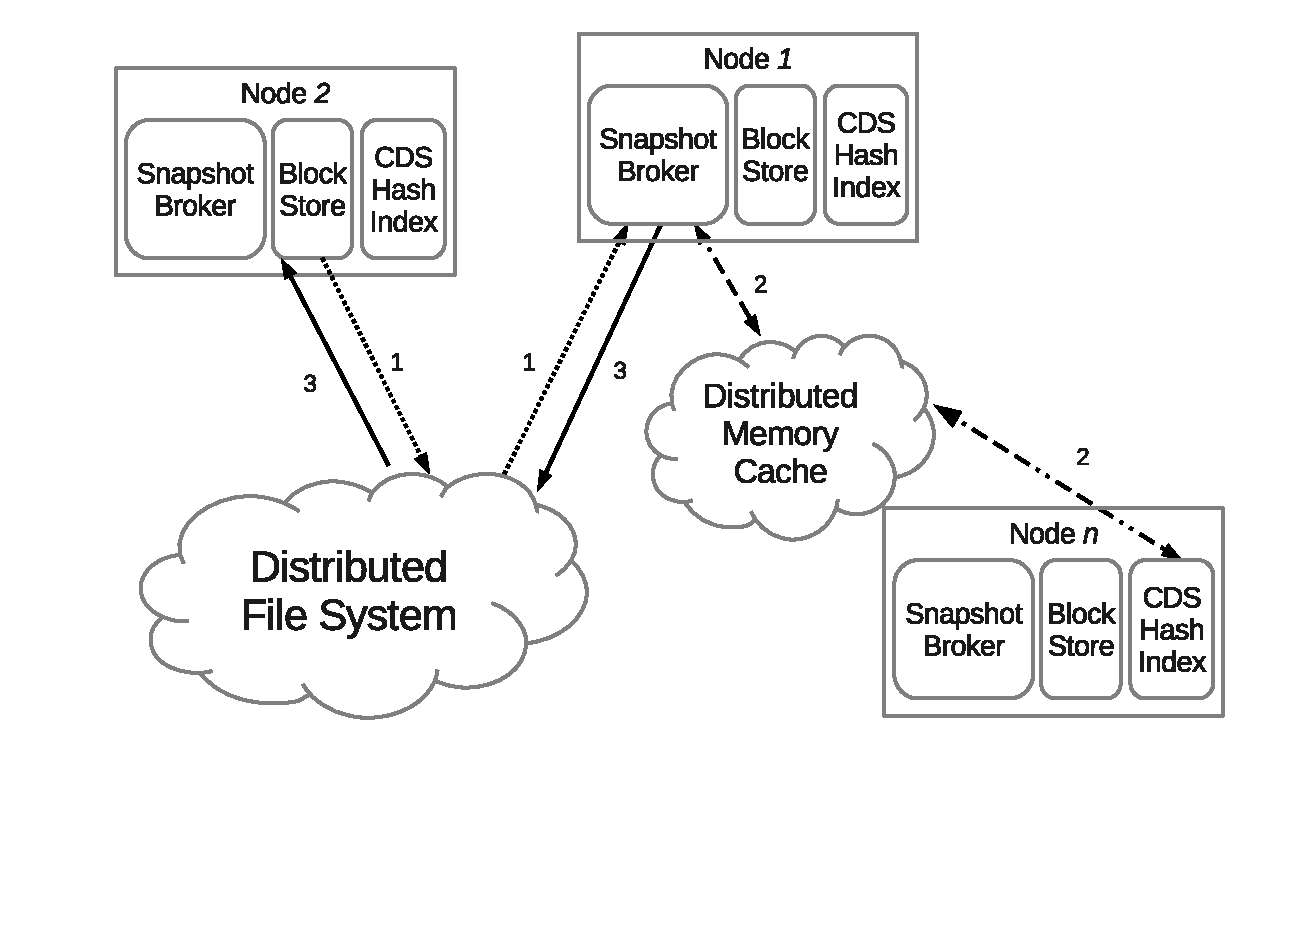
\epsfig{file=images/dedup_process.eps, height=2in, width=2.66in}
%  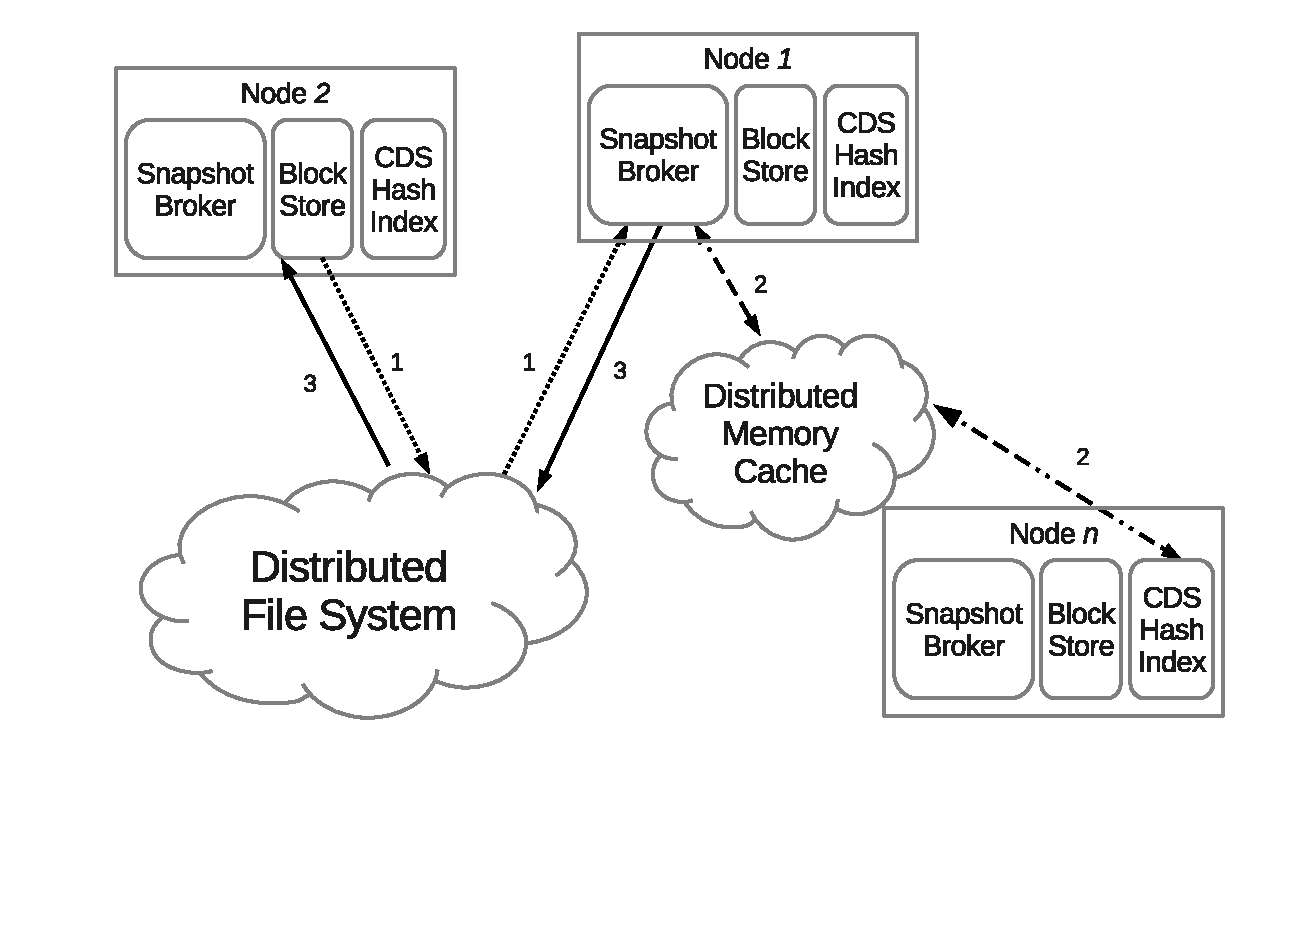
\epsfig{file=images/dedup_process.eps,  width=3.2in}
%  \caption{An example  of multi-level deduplication process.}
%  \label{fig:arch}
%\end{figure}

The inner VM deduplication contains two levels of duplicate detection efforts and the representation of
each snapshot is correspondingly designed as a two-level level index data structure in the form of a hierarchical
directed acyclic graph as shown in Figure~\ref{fig:snapshot}.
An image file is divided into a set of segments and each  segment contains hundreds of content blocks from the bottom level.
These blocks are of variable-size, partitioned using
the standard chunking technique~\cite{similar94} with 4KB as the average block size. 
%To simplify the deduplication process, segments are aligned to fix-sized boundaries, currently using 2MB.
Segment metadata (called segment recipe) records its  content block hashes and data pointers. 
The snapshot recipe contains a list of segments and other meta data information.
\begin{itemize}
\item {\em Level 1 Changed segment tracking}.
% If a segment is not changed, indicated by a dirty bit embedded in the virtual disk driver, its content blocks are not changed as well, thus its segment recipe can be simply reused. Operations at this level have almost no cost and most of unmodified data are filtered here. 
We start with the changed block tracking approach in a coarse grain segment level.
In our implementation with Xen on an Alibaba platform, the segment size is 2 MB
and the device driver is extended to support tracking changed segments using a dirty bitmap. 
Since every write for a segment will touch a dirty bit, the device driver maintains dirty bits in memory
and cannot afford a small segment size.
It should be noted that dirty bit tracking is supported or can be easily implemented in 
major virtualization solution vendors. For example,
the VMWare hypervisor has an API to let external backup applications know 
the changed areas since last backup. 
The Microsoft SDK provides an API that allows external applications to monitor 
the VM's I/O traffic and implement such changed block tracking feature.

\item {\em Level 2  Similarity guided segment comparison.}
% If a segment is modified, we perform fine-grained deduplication using content blocks of this segment to compared with 
% the same segment in
% the previous snapshot (also called parent snapshot). Partial duplication
% within the segment can be detected and eliminated. 
Since the best deduplication uses a non-uniform chunk size 
in the average of 4KB or 8KB~\cite{Jin2009},
we conduct additional local similarity guided deduplication on a snapshot by comparing
chunk fingerprints of a dirty segment 
with those in  {\em similar} segments from its parent snapshot. 
We define two segments are similar if their content signature is the same.
This segment content signature value is defined as the minimum value of all its chunk fingerprints 
computed during backup and is recorded in the snapshot metadata (called recipe). Note that this definition of
content similarity is an approximation~\cite{resemblance97}.  When processing a dirty segment,
its  similar segments can be found easily from the
parent snapshot recipe.  Then recipes of the similar segments are loaded to memory,
which contain chunk fingerprints to be compared.
To control the time cost of search, we set a limit on the number of  similar segments recipes to be fetched. 
For a 2MB segment, its segment recipe is roughly 19KB which contains about 500 chunk fingerprints and other chunk metadata,
by limiting at most 10 similar segments to search, the amount of memory for maintaining those similar segment recipes is small.
As part of our local duplicate search we also compare the current segment
against the parent segment at the same offset.

\end{itemize}

We choose this two-level structure because in practice we observe that during each backup period only a small amount
of VM data are added or modified. As the result, even the metadata of two snapshots can be highly similar,
thus aggregating a large number of content blocks as one segment can significantly
reduce the space cost of snapshot meta data. 
%Namely the  snapshort metadata starts with
%the representation of segment-level meta data. Each segment receipe can be further represented by
%a set of content block receipes.

How can we choose the length of a segment?
Instead of using variables-sized segments, we take a simple approach
to let every segment being aligned to the page boundary of each virtual image file.
For Aliyun, each VM image file is represented as a virtual disk file format
(called \emph{vhd} at Xen) and we use a dirty bit to capture if a page (or segment) of a virtual disk file 
has been modified or not to ease the segment-level deduplication.
%This is effective because  
%a vhd   file keeps the allocated inner blocks at the same positions until deletion,
%which means the locality of snapshot data is almost natively aligned. 
A dirty bit array is used to indicate which segments have been modified or not. 
Each page (segment) size in our implementation uses 2 MB, which contains a large number of content blocks.
%Enforcing a boundary at every 2MB will 
%only break 0.2\% of total data blocks which is tiny.
% dirty bits array. This is because
%Inside the TapDisk driver, we maintain an array of \emph{dirty bits} to record the dirty area
%of runtime VM image file since the last snapshot, each bit represent a 2MB fix-sized
%data segment. During a snapshot operation, we only need to look at the dirty region
%rather than scan over the whold image file, which would be extremely slow.


%We let each virtual disk has its own block store rather than sharing for several reasons:
%first, all data written to block store are already being processed by deduplication
%process, thus no sharing is necessary unless we want to perform additional deduplication
%inside the block store. Second, such seperation will facilitate VM data stastics, 
%deletion and migration. Finally, this reduces the complexity of concurrent snapshot operations.

Once level-2 deduplication is activated for those segments that have been modified,
it requires memory to load  block fingerprints from the corresponding
parent snapshot's segment.
This scheme processes one segment at time and each segment of 2 MB contains about 
500 content blocks on average given 4KB is the average block size.
That only takes a tiny amount of space to hold their fingerprints.
%Given  1-2 hours of window to backup snapshots and every VM has  on average about 40GB, there is enough
%time to search all segments sequentially~\cite{NOT-CLEAR-HERE}

\subsection{Popularity guided Cross-VM Deduplication with PDS}
\label{sect:crossVM}

The level-3 deduplication is to identify duplicated data blocks among multiple VMs through the index cache
of popular data set (PDS).  PDS is the most popular content blocks 
among snapshots across all VMs. 
Each index entry contains  the block fingerprint and a reference pointer to the location of its real content
in the snapshot content block store.
%The structure of PDS meta is not different from the segment recipe we discussed above, 
%except that it is partitioned into many small slices so that each node is easy to load its own slice. 

At the runtime, the PDS index resides in a distributed  memory lookup table  
implemented using Memcached~\cite{memcached} to leverage the aggregated memory in a cluster.
The usage of memory at each machine is small and thus  this scheme  does not
lead to  a memory resource contention with the existing cloud services.
PDS raw data stored  in the distributed file system
has multiple copies in different machines for the purpose of fault tolerance and 
while providing high read throughput.  

To control the size of searchable popular data in this global setting, we focus on those items that 
are most popular based on the historical snapshot data and the popular analysis is conducted periodically to ensure 
meta data freshness to match the latest data access trend.
There are two advantages to exploit this.
First, a smaller PDS reduces overall resource requirement while covering most of data duplication.
Second, knowing this small set of data is shared heavily makes the fault tolerance management 
easier because we can replicate more copies to mitigate the failure.

\begin{figure}[htbp]
\centering
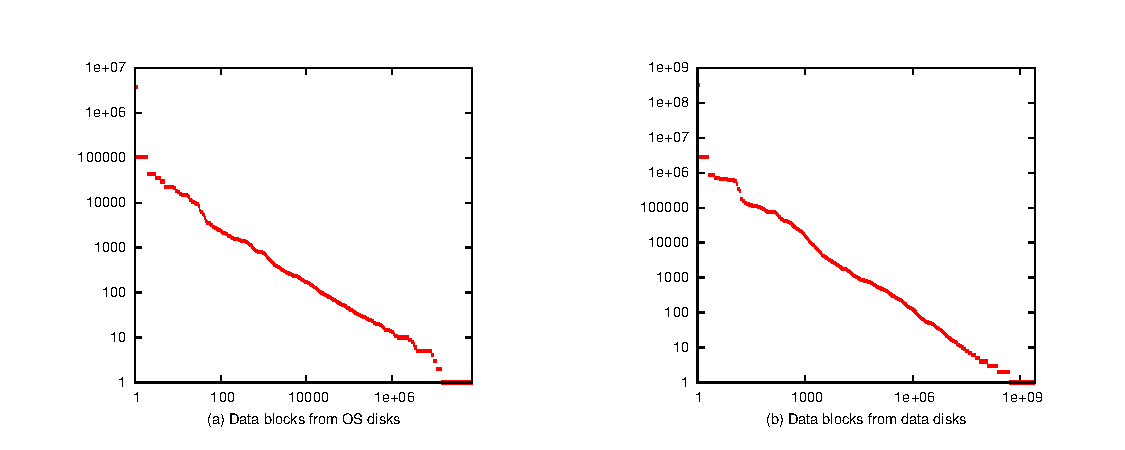
\includegraphics[width=5in]{images/vector.pdf}
\caption{Number of duplicates vesus ranking}
\label{fig:zipf-data}
\end{figure}

In Aliyun's VM cloud, each VM explicitly maintains  one OS disk, plus one or more data disks.
During VM's creation, its OS disk is directly copied from user's chosen base image.
Given the separation of OS disks and data disks, we study  their characteristics separately.
We expect that data related to OS and popular software installations are not frequently
modified or deleted, to facilitate analysis we call them \emph{OS-related} data, 
and the rest of data, either from OS or data disks, are called \emph{user-related} data.
%base image data as a hint.Through users may change configurations, install software, or write user data into OS disk,
%Thus most of content blocks for the OS related snapshots  shall keep unchanged.
%This is verified in  Section~\ref{sect:exper}.

We have studied the popularity of popular blocks in the OS and data disks from a dataset
containing over 1,000 VMs, taking their first snapshots to watch the cross-VM duplication pattern 
(scale of OS disk sampling is smaller due to performance impact to user VMs).
Figure \ref{fig:zipf-data} shows the duplicate count for unique data blocks sorted by their ranking in 
terms of the duplication count. $Y$ axis is the popularity of a data block in a log scale 
measured its duplicate count among snapshots. $X$ axis is the identification of data blocks in a log scale
sorted by their duplicate rank.  The rank number 1 is the block with the highest number of duplicates.
These two curves exhibit that the popularity of popular blocks partially follows a Zipf-like distribution.
%$Y$ axis is the popularity of an OS block in a log scale 
%measured its duplicate count among snapshots. $X$ axis is the identification of OS blocks in a log scale
%sorted by their duplicate rank.  
%For the top ranked blocks, there is a flat line in terms of duplicate counts. That
%is because there are a large number of OS blocks which have appeared in all copies of such OS releases.




%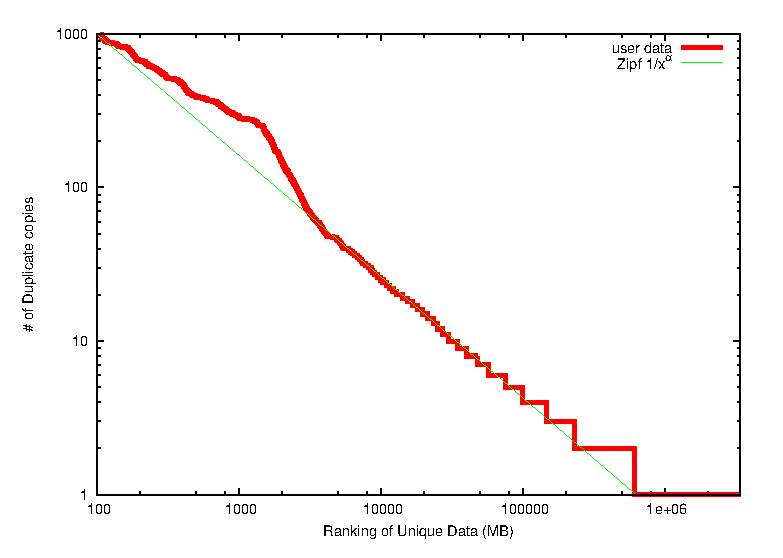
\epsfig{file=images/log-log.disk.eps, width=3in}

%\begin{tabular}{cc}
%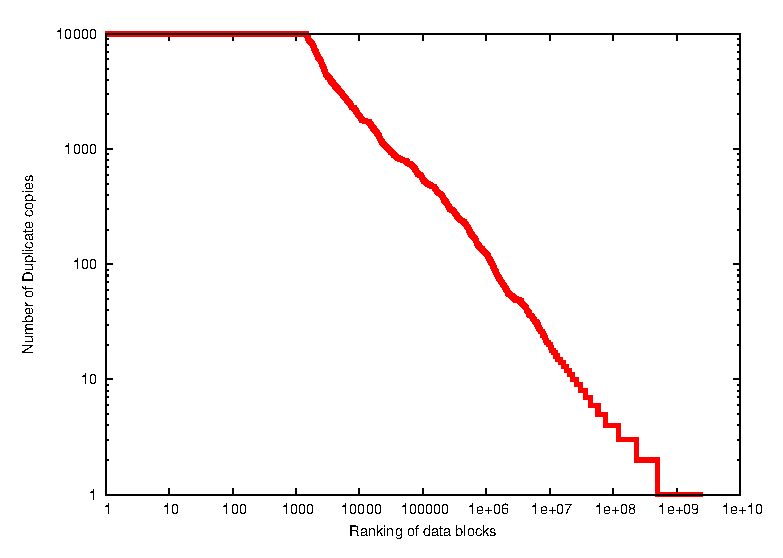
\epsfig{file=images/datadisk.count_rank.eps, width=1.5in} &
%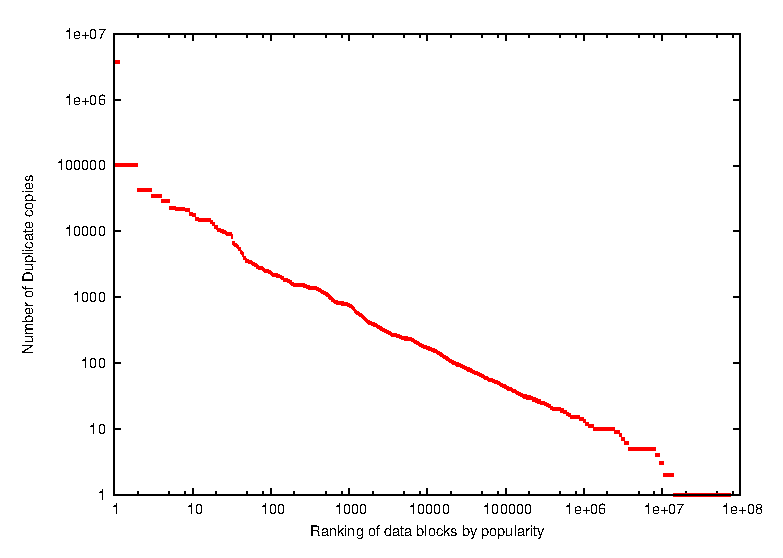
\epsfig{file=images/35vmos.count-rank.eps,width=1.5in}
%\end{tabular}


%\begin{figure}
%\centering
%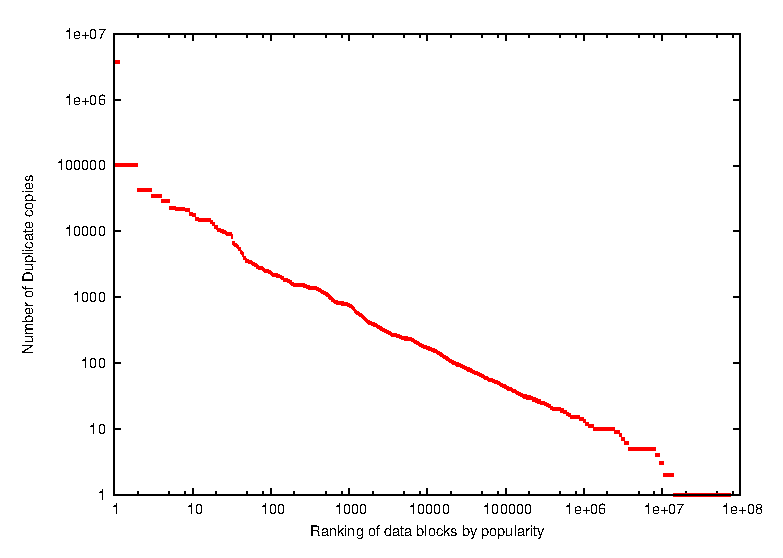
\epsfig{file=images/35vmos.count-rank.eps,width=3in}
%\caption{ Duplicate count of  popular OS blocks in a log scale.}
%\label{fig:OSpopular}
%\end{figure}

Base on the Zipf-like distribution pattern, many previous analysis and results on web caching\cite{Adamic2002,Breslau1999b} may apply.
In general this indicates a small set of popular data dominates data duplication.
Although we already know OS-related data are heavily duplicated among OS disks, 
it still surprises us that user-related data follow a similar pattern.
Therefore, we collect the PDS by performing global reference counting through map-reduce for all
blocks in snapshot store, and select the most popular ones base on the memory limitation of
PDS hash index. 

The PDS collected from user-related data is generally proportional to the data size.
As discussed in Section~\ref{inline:impl}, selecting about 1\% of data (after level 1 and level 2 deduplication)
can cover about 38\% of data blocks. Consider we allow maximum 25 VMs per machine, each VM has
about 30 GB of user-related data, having 10 snapshots in its snapshot store and the data change ratio during
each backup is 10\%, this translates to 15 GB PDS data per machine. 
Consider each PDS hash index entry cost about 40 bytes and the average block size is 4KB, this leads to
a 1:100 ratio so the 
memory cost by PDS hash index is about 150 MB per machine.
On the other hand, the PDS from OS-related data is only relevant to the number of OS releases.
Our experiment on 7 major OS releases shows that about 100 GB of data is never modified, and we expect
it won't grow over 200 GB in the near future. So it would cost the entire cluster 2 GB of memory to
store its hash index, or 20 MB per machine on a 100 node cluster. On average each OS disk has about 10 GB
of data that can be completely eliminated in this way.
Thus in total the PDS index size per node takes less than 170 MB in a large cluster bigger than 100 nodes, 
covering over 47\% of blocks in OS and data disks after inner-VM deduplication.
This memory usage is well below the limit required by our VM services.

\subsection{Illustration of multi-level deduplication process}

%%Our deduplication process is divided into three levels, at each level, we eliminate the most of duplicate data with available knowledge, preventing them from going further because deduplication at deeper level is more expensive.
%
\begin{figure}
  \centering
  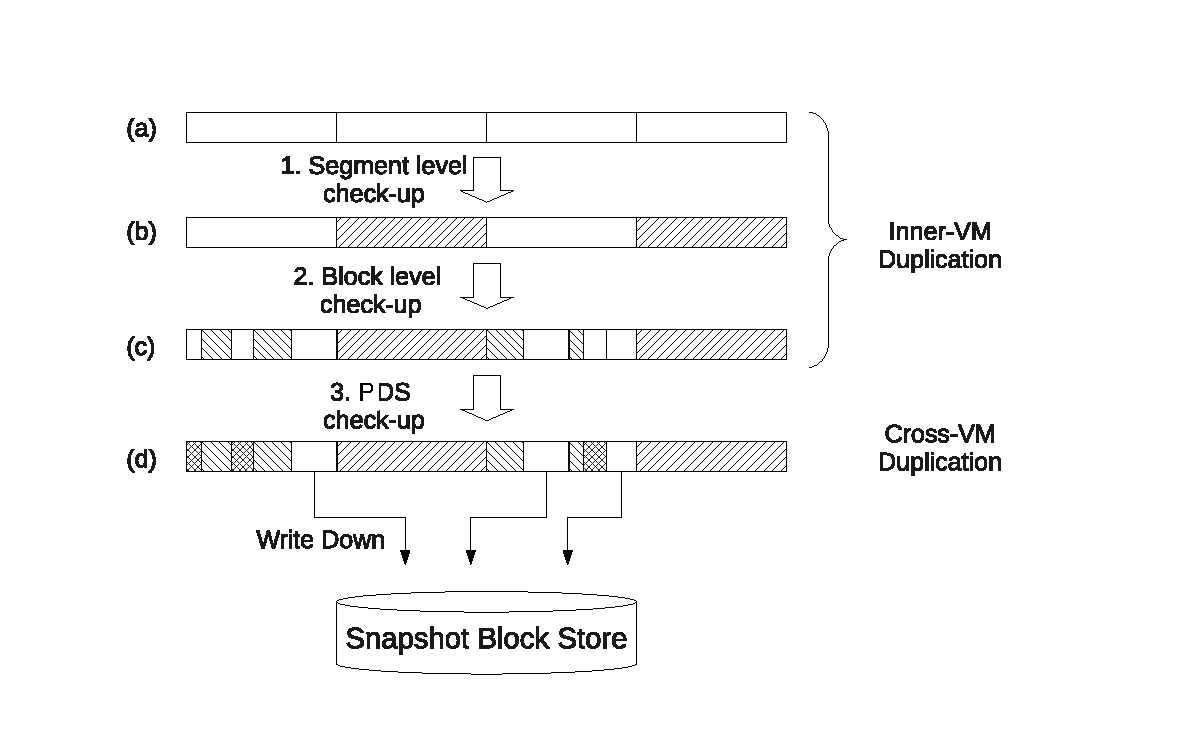
\includegraphics[width=5in]{images/dedup_flow2.pdf}
  \caption{Illustration of snapshot deduplication dataflow.}
  \label{fig:dedupflow}
\end{figure}

We illustrate the steps of 3-level deduplication in Figure~\ref{fig:dedupflow}, which can be summarized as 5 steps:
\begin{enumerate}
\item {\em Segment level checkup.}
As shown in Figure~\ref{fig:dedupflow} (a),
when  a snapshot of a plain virtual disk file is being created, we first check the dirty bitmap 
to see which segments are modified. If a segment is not modified since last snapshot, 
it's data pointer in the recipe of the  parent snapshot  can be directly copied into 
current snapshot recipe (shown as the shadow area in Figure~\ref{fig:dedupflow} (b)).

\item {\em Block level checkup.}
As shown in Figure~\ref{fig:dedupflow} (b),
for each dirty segment, we divide it into variable-sized blocks,
and compare their signatures with  the similar segment recipes in the previous snapshot (called parent
snapshot). 
For any duplicated block, we copy the data pointer directly from the parent segment recipe. 
\item {\em PDS checkup.} For the remaining  content blocks whose duplicate status is unknown,
Figure~\ref{fig:dedupflow} (d)
shows  a further check to compare  them with  the cached signatures in the PDS by querying
the PDS hash index. If there is a match, the corresponding data pointer from the PDS index is
copied into the segment recipe. 
\item {\em Write new snapshot blocks :}
If a data block cannot be found in the PDS index, this block is considered to be a new block
and such a block is to be saved in the snapshot store, the returned data pointer is
saved in the  segment recipe.
\item {\em Save recipes.} Finally the  segment recipes are saved in the  snapshot block store also.
 After all segment recipes are saved, the snapshot recipe is complete and can be saved.
\end{enumerate}

If there is no parent snapshot available, which happens when a VM creates its first snapshot, 
only PDS-based checkup will be conducted. 
Most of the cross-VM duplication, such as OS-related data, is eliminated
at this stage. 


\section{System Implementation and Experimental Evaluations}
\label{inline:impl}
We have implemented the snapshot deduplication scheme on the Aliyun's cloud platform.
Objectives of our experimental evaluation are:
1) Analyze the popularality of content data blocks and the popularity  of hot items. 
2) Assess the effectiveness  of 3-level deduplication for reducing the storage cost of snapshot 
backup. 
3) Examine the impacts of PDS size on deduplication ratio.

\subsection{Experimental setup}

At Aliyun our target is to backup cluster up to 1000 nodes
with 25 VMs on each.
%We are running our deduplication/backup  service on 100 nodes.
%Memory usage is about 150MB space per node during backup and
%the CPU usage is very small during the experiments. 
Based on the data studied,  each VM has about  40 GB of storage  data usage on average,
OS disk and data disk each takes about 50\% of storage space.
The backup of VM snapshots is completed within two hours every day,
and that translates to a backup throughput of 139 GB per second, or 500TB per hour.
For each VM, the system keeps 10 automatically-backed snapshots in the storage while
a user may instruct extra snapshots to be saved.

% the system must finish saving daily snapshots of all VMs in 2 hours. In our typical 1000 nodes cluster, each node hosts 25 VMs, each VM has 40GB of data on average, that translates to backup throughput of 139GB/second, or 500TB/hour.

%In our snapshot deduplication architecture, PDS is the key to achieve greater deduplication than
%incremental backup solutions. Our basic assumption of PDS us that VM disks, especially OS disks,
%have huge amount of data in popular, and such popular data can be represented by a relatively smaller data set
%because of their high appearence frequency. As a result, the major portion of snapshot deduplication effect shall 
%emerge from eliminating the duplication of such a small data set. In this section, we evaluate
%the effectiveness of PDS using real user VM disks from our production VM cluster.

Since it's impossible to perform large scale analysis without affecting the VM performance,
we sampled two data sets from real user VMs to measure the effectiveness of our deduplication scheme.
Dataset1 is used study the detail impact of 3-level deduplication process,
it compose of 35 VMs from 7 popular OSes: 
Debian, Ubuntu, Redhat, CentOS, Win2003 32bit, Win2003 64 bit and Win2008 64 bit. For each OS, 
5 VMs are chosen, and every VM come with 10 full snapshots of it OS and data disk. 
The overall data size for this 700 full snapshots is 17.6 TB.

Dataset2 contains the first snapshots of 1323 VMs' data disks from a small cluster with 100 nodes. 
Since inner-VM deduplication is not involved in the first snapshot, this data set helps us to 
study the PDS deduplication against user-related data. The overall size of dataset2 is 23.5 TB.

All data are divided into 2 MB fix-sized segments and each segment is divided into 
variable-sized content blocks ~\cite{similar94,rabin81} with an average size of 4KB.
The signature for variable-sized blocks is computed using their SHA-1 hash. 
Popularity of data blocks are collected through global counting 
and the top 1\% will fall into PDS, as discussed in Section~\ref{sect:crossVM}.


%To compare the effectiveness with a full deduplication approach with an approximation,
%we use  extreme binning and perfect deduplication~\cite{extreme_binning09}. 
%For perfect deduplication and extreme binning, each snapshot is also divided into chunk blocks
%using TTTD with an average size of 4KB. The original extreme binning work uses the whole file
%as the input unit and  this size is too big in our system. 
%Thus we split each image snapshot file into variable-sized segments base on the block hash list, 
%using TTTD with average size of 2MB.

\subsection{Effectiveness of Multi-level Deduplication}

\begin{figure}
  \centering
  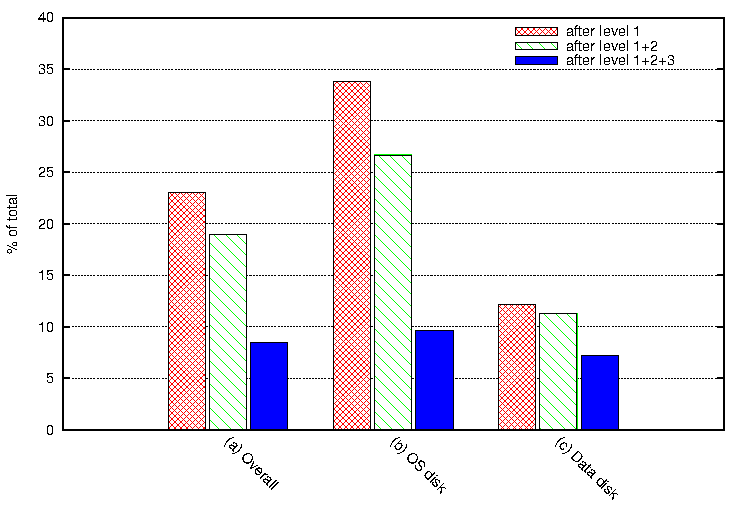
\includegraphics[width=5in]{images/overall_effect.pdf}
  \caption{Impacts of 3-level deduplication. The height of each bar is the data size after 
deduplication divided by the original data size and the unit is percentage. }
  \label{fig:overall}
\end{figure}

Figure~\ref{fig:overall} shows the overall impact of 3-level deduplication on dataset1.
The X axis shows the overall impact in (a),  impact on OS disks in (b), and impact on data disks in (c).
Each bar in the Y axis shows the data size after deduplication divided by the original data size.
Level-1 elimination can reduce the data size to about 23\% of original data, namely it delivers close 77\% reduction.
Level-2 elimination is applied to data that could pass level-1, it
reduces the size further to about 18.5\% of original size, namely it delivers additional 4.5\% reduction.
Level-3 elimination together with level 1 and 2
reduces the size further to 8\% of original size, namely it delivers additional 10.5\% reduction.
Level 2 elimination is more visible in OS disk than data disk, because data change frequency is really small
when we sample last 10 snapshots of each user in 10 days. Nevertheless, the overall impact of level 2 is still significant.
A 4.5\% of reduction from the original data represents about 450TB space saving for a 1000-node cluster.


\begin{figure}
  \centering
 %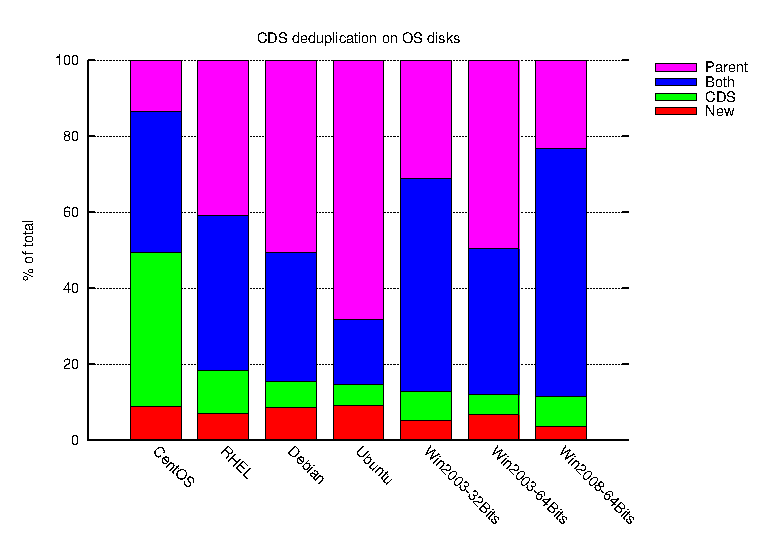
\epsfig{file=images/os_cds_sim.eps, width=3in}
  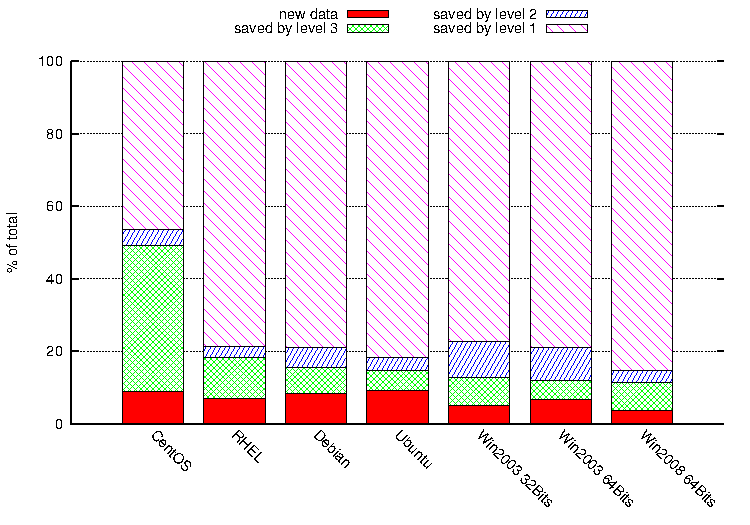
\includegraphics[width=5in]{images/3level_os.pdf}
  \caption{Impact of 3-level deduplication for OS releases.}
  \label{fig:oscds}
\end{figure}

%To see the impact of multi-level deduplication on different OS releases,
%Some of  OS disks are modified frequently and in some cases,  users even store a large amount of user data on
Figure~\ref{fig:oscds} shows the impact of different levels of deduplication for different OS releases.
In this experiment, we tag each block in 350 OS disk snapshots from dataset1 as  ``new''
if this block cannot be deduplicated by our scheme and thus has to be written to the snapshot store;
``PDS''  if this block can be found  in PDS;
``Parent segment'' if  this block is marked unchanged in parent's segment recipe.
``Parent block'' if  this block is marked unchanged in parent's block recipe.
With this tagging, we compute the percentage of deduplication accomplished by each level.
As we can see from Figure~\ref{fig:oscds}, level-1 deduplication accomplishes a large percentage of elimination,
this is because the time interval between two snapshots in our dataset
is quite short and the Aliyun cloud service makes a snapshot  everyday  for each VM.
On the other hand,  PDS still finds lots of duplicates that inner VM deduplication can't find,
contributing about 10\% of reduction on average.

It is noticeable that level-1 deduplication doesn't work well for CentOS, a significant percentage of data is not
eliminated until they reach level-3. It shows that even user upgrade his VM system heavily and frequently
such that data locality is totally lost, those OS-related data can still be identified at level-3. 

In general we see a stable data reduction ratio for all OS varieties, ranging from 92\% to 97\%, that means
the storage cost of 10 full snapshots combined is still smaller than the original disk size. And compare to 
today's widely used copy-on-write snapshot technique, which is similar to our level-1 deduplication, our
solution cut the snapshot storage cost by 64\%.


%Combining OS disks in all the VMs, we see the overall 7.4TB of data is reduced to 512GB. 
%The extreme binning approach can reduce this data set to 542GB, which is slightly worse. As a reference, 
%perfect deduplication achieves 364GB in this experiment.

%Overall speaking, inner   VM deduplication or  PDS-based deduplication
%can work well alone, but by combining them together we get a fairly good and stable deduplication ratio to 
%all kind of OSes. 
%Compared to a traditional dirty bit approach based on pages of
%each file (e.g. segment in our scheme),
%our PDS-based level 3 approach  can save additional 50\% storage space because many of level 2 block
%content can be eliminated using the PDS also.

\subsection{Coverage of popular data blocks}

%We study characteristics of popular data blocks among snapshots of VM users
%and examine the impacts if we only store a relative small amount of popular data blocks to be sored in the PDS server.
%There are two advantages to exploit this.
%First, a smaller PDS reduces overall resource requirement while covering  most of data blocks in snapshots.
%Second a smaller PDS makes the fault tolerance management  easier because we can replicate  more copies
%to mitigate the failure.

%We consider each virtual disk contains two parts: OS partition and regular user data partition
%and study their characteristics seperately.
%In Aliyun's VM cloud, each VM explicitly maintains  one OS disk, plus  one or more data disks.
%During VM's creation, its OS disk is directly copied from user's choosen base image.
%Since  they dare brought by the operating system and popular 
%software installations,  they are rarely modified or deleted.
%base image data as a hint.
%Through users may change configurations, install software, or write user data into OS disk,
%but most of the OS related data shall keep unchanged. 

%Previous study has also supported this\cite{vmimage}. Therefore, we can let all OS disks share these
%popular data in their snapshot backups.
%We choose user's data disks rather than OS disks in thie experiment for several reasons: First, the data in OS disks are 
%instinctively highly similar, because most of the VM users only make some popular or unique but tiny changes to their OSes,
%so the data duplication pattern in OS disks cannot reflect the real distribution of general user data.
%Second, the data disks are way more important in terms of data safty and backup because they are 
%what users really care about.

%Furthermore, our study on user's data disks has shown that the duplication pattern of
%variable-sized data blocks follows \emph{Zipf-like} distribution. As a result, the major portion of 
%deduplication effect will emerge from eliminating the duplication of frequently seen data.
%define PDS
 
\begin{figure}
\centering
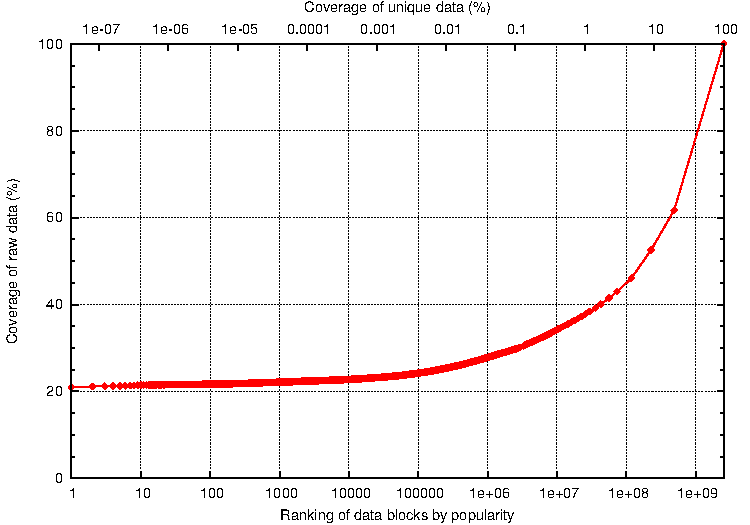
\includegraphics[width=5in]{images/ay41a_big_data_disk_cdf.pdf}
\caption{Cumulative  coverage of popular popular user data blocks.}
\label{fig:userdatacoverage}
\end{figure}

One of our biggest advantage is small memory footprint for deduplication, because we only
eliminate a small amount of highly popular data.
we use dataset2 to demonstrate the coverage of popular data blocks on user-related data, 
as shown in Figure \ref{fig:userdatacoverage}.
%content blocks used in image files using 90\% of
%the collected dataset.
%Figure \ref{fig:userdatacoverage} shows the cumulative coverage  ratio of  popular popular user data blocks. 
The $X$ axis is the rank of popular user data blocks, and $Y$ shows how much raw data can be covered given
the size of PDS.
Let $S_i$ and $F_I$ be the size and duplicate count 
of the $i$-th block ranked by its duplicate rank.  Then $Y$ axis is the coverage of
the popular dataset covering data items from rank 1 to rank $i$. Namely  
\[
\frac{ \sum_{i=1}^{i} S_i * F_i} {\mbox{Total data size}}.
\]

Thus with about 1\% of blocks on data disks, PDS can cover about 38\% of total data blocks
appeared in all data snapshots. The corresponding PDS index uses no more than 150 MB memory per machine,
which can be easily co-located with other cloud services.

%Figure~\ref{fig:OSdatacoverage} shows the cumulative coverage  ratio of  popular popular OS blocks. 
%From both graphs, a small number of most popular popular blocks can coverage a large percentage of 
%snapshot blocks and thus the size of PDS can be chosen to be small while still having a large
%coverage. 

%\begin{figure}
%\centering
%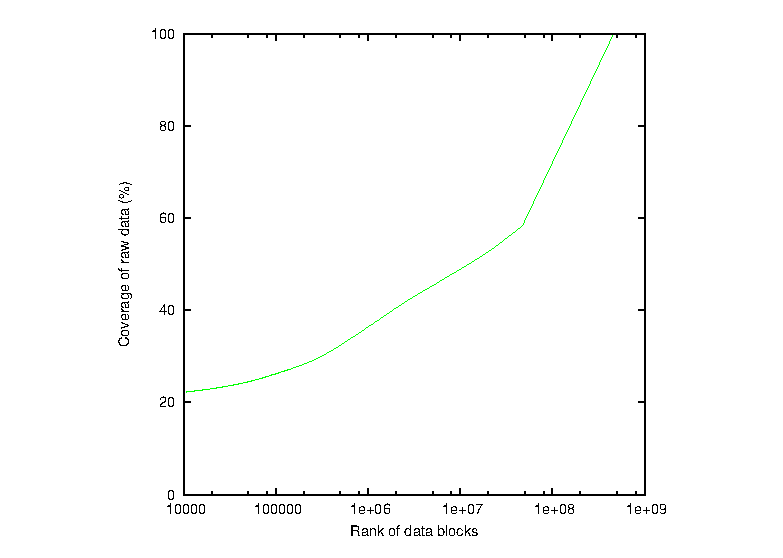
\epsfig{file=images/ay41a_small.os_incremental.cdf.eps, width=3in}
%\caption{ Cumulative  coverage of popular popular OS disk blocks.}
%\label{fig:OSdatacoverage}
%\end{figure}


%We define \emph{OS PDS} to be the unchanged data across the base VM image and the snapshots of all
%OS disks which are derived from it. Such data are brought by the operating system and popular 
%software installations, they are rarely modified or deleted, and can be easily extracted using 
%base image data as a hint.


Because there are a limited number of OS releases, we study popular blocks among
OS disks loaded with  the same OS release. 
%The selection of PDS is completed by separating OS disk and data disk.
%While block popularality among data disks may be affected in some degree
% when we scale up the number of total VMs  to be supported,
%we expect that  the block popularality among OS disks still remains to be high and  
%%can be well covered by a fixed PDS because users still adopt popular OS releases.
%we choose 7 major OSes in Aliyun's
%VM cloud platform and they are: 
%Win2008 Server 64 bits, Win2003 Server 32 bits, Win2003 Server 64 bits, RHEL, CentOS, Ubuntu Server and Debian (all Linux
%distributions are 64 bits).
%we examine 5 VM user disks from each OS, and 10 snapshots for each VM. These VMs have been actively used by their
%owners. Some of  OS disks are modified frequently and in some cases,  users even store a large amount of user data on
%their OS disks. 
%For example, some Ubuntu OS disks have only 2GB of data while some have 50GB.
%For each OS, the base image and all OS
%disk snapshots are divided into variable-sized blocks. Then 
In  Figure~\ref{fig:OSunchanged},  we list a conservative  popularality study in 7 major OS versions  supported
in Aliyun.
%We consider the earlier snapshot for each OS disk as the base image.
For every block in the base image, we classify this block as ``unchanged''
if this block has appeared in all snapshots of the same OS release even they are used by different VMs.
Figure \ref{fig:OSunchanged} shows that for each
OS,  at least 70\% of OS blocks are completely unchanged among all snapshots of the same OS. 
Some latest release  of OS tends to have a higher percentage of content change
while  old release tends to have more variations of content versions.
That can be interpreted as that users with very old  version of operating systems
have a lower tendency to update their OS versions and this causes a larger discrepancy
among OS snapshots of these users.

%into the unchanged category of OS data.

\begin{figure}
\centering
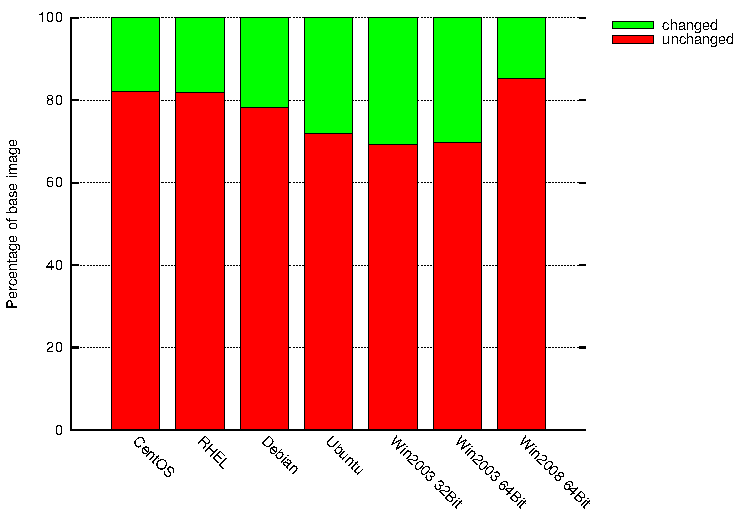
\includegraphics[width=5in]{images/os_subset.pdf}
\caption{Percentage of completely popular blocks among different VMs for the same OS release.}
\label{fig:OSunchanged}
\end{figure}

Based on the above analysis, we have selected a small set of most popular
OS blocks, which is about 100 GB OS data and its corresponding PDS index takes about 1 GB memory space in total.
They can cover sufficiently over 70\% of OS-related data.

%Then we use this PDS to run the deduplication process again.
%That correspond to about  80GB of OS blocks and its corresponding PDS meta occupies 800MB in the cache.
%  data from 350 OS disk snapshots,

%The above analysis is only an estimation of OS and software related popular data, 
%some user installed software may not be discovered by this method because they are not 
%included in the base image. However, as we can see in the next section, 
%the overall duplication of user generated data
%follows the Zipf-like distribution, thus all popular data can be discovered by statistic analysis.


%Zipf's law has been shown to characterize use of words in a natural language, city populations, 
%popularity of website visits and other internet traffic data.

%Here we present the first fully consistent empirical study showing that data duplication
%pattern in very large scale storage follows Zipf-like distribution. More specifically,
%we show that the duplication count of any unique data block is inversely proportional to its rank
%in the frequency table, with $\alpha$ smaller than unity. 
%As far as we know, this is the first study of large scale real user data to disclose
%the Zipf-like distribution pattern in data storage area.

%\subsubsection{The model}
%Consider a general storage system that holds user's files without any deduplication. 
%Let $N$ be the total number of unique data blocks after 
%content-defined chunking and deduplication, 
%$C_N(i)$ be the number of duplicate copies that the $i$th data block being
%stored in storage, given all the unique data blocks be ranked in order of their number of duplicate copies.
%Let $S_i$ be the size of $i$th block,
%then the actual ranking of the $i$th block is reflected by $\sum_{1}^{i-1}S_i$. 

%\subsubsection{Methodology}
%1323 users' virtual data disks were scanned using TTTD content-defined chunking, and we performed global perfect deduplication 
%to caculate the number of duplicate copies of each individual unique block. We choose 2KB, 4KB, 16KB as the minimum, average
%and maximum block size, all variable-sized blocks are compared by their SHA-1 hash arther than real data.
%
%We choose user's data disks rather than OS disks in thie experiment for several reasons: First, the data in OS disks are 
%instinctively highly similar, because most of the VM users only make some popular or unique but tiny changes to their OSes,
%so the data duplication pattern in OS disks cannot reflect the real distribution of general user data.
%Second, the data disks are way more important in terms of data safty and backup because they are 
%what users really care about.

%In our snapshot deduplication architecture, PDS is the key to achieve greater deduplication than
%incremental backup solutions. Our basic assumption of PDS us that VM disks, especially OS disks,
%have huge amount of data in popular, and such popular data can be represented by a relatively smaller data set
%because of their high appearence frequency. As a result, the major portion of snapshot deduplication effect shall 
%emerge from eliminating the duplication of such a small data set. In this section, we evaluate
%the effectiveness of PDS using real user VM disks from our production VM cluster.


\subsection{A comparison of perfect and PDS-based deduplication }
%Figure~\ref{fig:pd} shows the compression ratio of perfect deduplication at different dataset sizes
%as we vary the data size from about 4 terabytes to about 23.5 terabytes.
After level-1 and level 2 elimination, we find that 
the complete deduplication would reduce the storage cost further by 50\%. 
If we put all these unique data into PDS, 
we could achieve complete deduplication,
but fingerprint lookup in such huge PDS hash index would become a bottleneck as discussed in many pervious works. 
So we use dataset2 to evaluate how much space saving of 
deduplication can be achieved when varying the PDS size.
%\begin{figure}
%  \centering
%  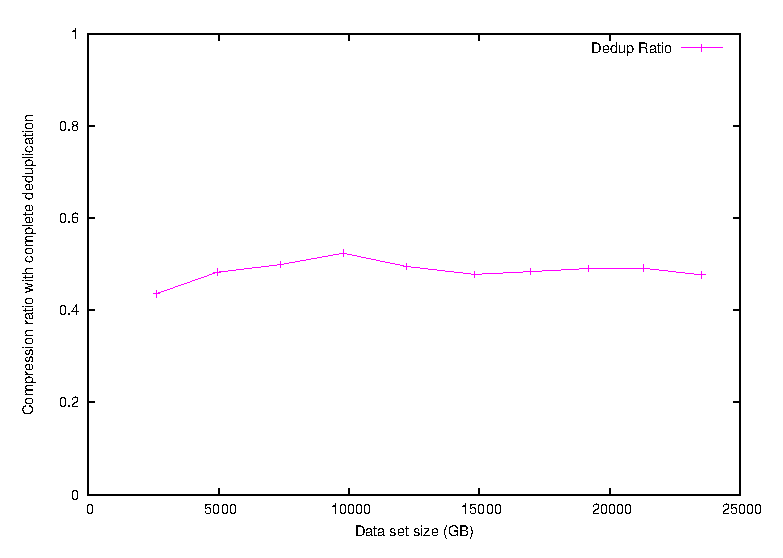
\epsfig{file=images/dedup_ratio.eps, height=2in, width=2.66in}
%  \caption{Perfect deduplication on data disks}
%  \label{fig:pd}
%\end{figure}

%We rank unique data blocks by their duplication count, and choose the hottest blocks as PDS. 
Figure \ref{fig:datacdssize} shows the relationship between PDS cache size and relative space saving ratio
compared to the full deduplication.  The unit of PDS size is gigabytes.
We define \emph{space saving ratio} as the space saving of PDS method divided by 
full deduplication space reduction. 
With a 100 GB PDS data (namely 1 GB PDS index) can still  accomplish about 75\% 
of what perfect deduplication can do.
%But this effect decreases when more data are added to PDS. 
%The lower bound of PDS space saving ratio is 50\%, which is very easy to accomplish. 

\begin{figure}
  \centering
  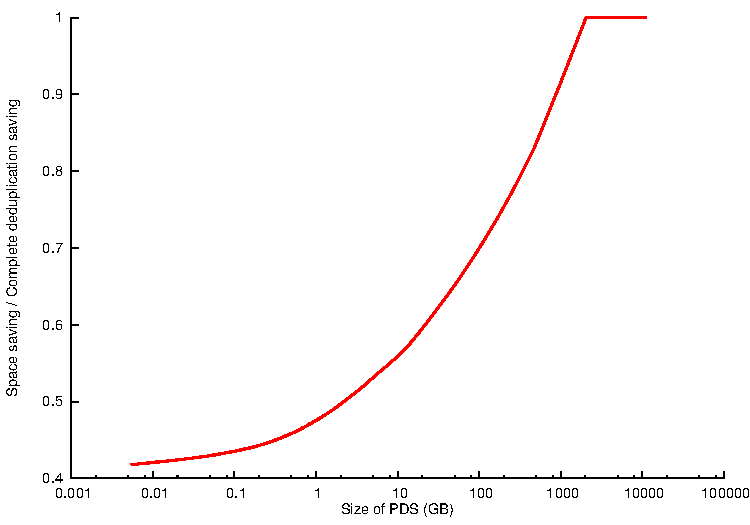
\includegraphics[width=5in]{images/uniquedata-saving1.pdf}
  \caption{Relative ratio of space size compared to full deduplication when PDS size changes.}
  \label{fig:datacdssize}
\end{figure}

%PDS size is restricted by system memory resource.
With dataset2, Figure \ref{fig:datacds} shows how PDS space saving ratio
compared to the full deduplication is affected by the dataset size. 
%The calculation is done after level 1 and level 2 deduplication.
In this experiment we first set out a goal of space saving ratio completed, 
then watch how much data needs to be placed in PDS cache to achieve this goal.
From the graph we can see a 75\% saving ratio lead to a stable ratio between 
PDS size and data size, which requires 1\% of data to be placed in PDS.

When we deal with a large cluster of 1,000 nodes, we expect that using
1\% of data disks can cover more than what we have seen from this
1323 VM dataset, assuming that the average behavior of every subcluster with 100 machines
exhibits a similar popularality. 
In addition to this, PDS for OS disks will become even more effective when
there are more VMs sharing the same collection of OS releases. 
%Base on above data we can estimate the size of data PDS and its effect. 
%Currently we prepared 500MB memory per machine to store PDS meta, then it can represent 50GB of data. 
%If we assume each VM has 30GB of user data at runtime, and we host 25 VMs per machine, 
% maintain 10 snapshots per VM, each brings 10\% additional modified data. 
%Thus the user data in snapshot system is 1.5TB per machine. So the upper bound of 
%$PDS size/ Data size = 0.033$, which is sufficient for the 75\% saving goal.

\begin{figure}
  \centering
  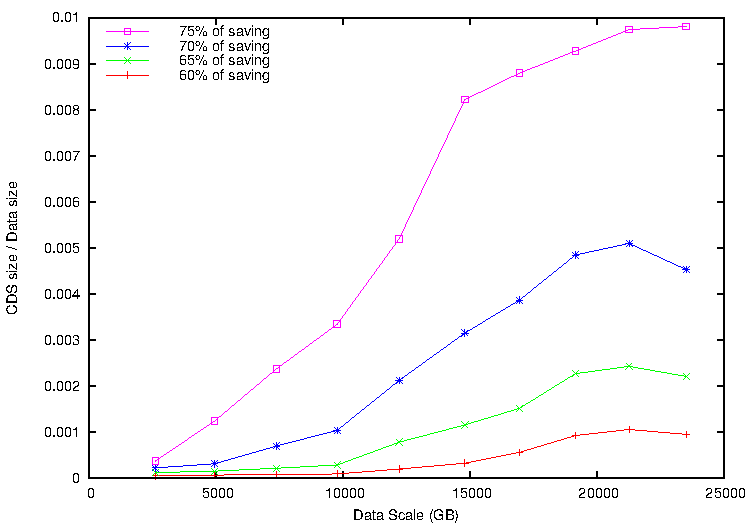
\includegraphics[width=5in]{images/cds_scale_07.pdf}
  \caption{The relative size ratio of  PDS over the data size. }
  \label{fig:datacds}
\end{figure}

\section{Related Work}
\label{inline:related}
In a VM cloud, several operations are provided for creating and managing snapshots and snapshot trees,
such as creating snapshots, reverting to any snapshot, and removing snapshots.
For VM snapshot backup, file-level semantics are normally not provided. 
Snapshot operations are taken place at the virtual device driver level, which means no fine-grained file system metadata can be used to determine the changed data. Only raw access information at disk block level are provided.
%Snapshots may be shared among VMs when a user runs the same binary image on different  VMs.
% This feature complicates the snapshot management, 
%but also require all snapshots be managed in a global namespace.


%While snapshot backup loads are heavy but computing and storage  resources available 
%can be limited to reduce the overall operation cost of a cloud. The whole VM cluster have petabytes of data and need to 
%be backed up at daily basis, if not more frequently. But at the same time snapshot tasks must not affect the normal VM operations
%in a cloud service, which means only a tiny slice of CPU and memory can be used for this purpose.


VM snapshots can be  backed up  incrementally by identifying file  blocks that have
changed from the previous version of the snapshot~\cite{Clements2009,Vrable2009,TanIPDPS2011}.
%Even though the snapshots are saved incrementally,
%when deleting a snapshot, only the data not needed for any other snapshot is removed.
%So regardless of which prior snapshots have been deleted, all active snapshots will contain
%all the information needed to restore the virtual disk.
%One widely used snapshot strategy is copy-on-write (CoW).
%The earlier use of COW is to improve memory usage and reduce copying overhead in process 
%management~\cite{OSbook,Waldspurger2002} and it can be extended for snapshot 
%storage management~\cite{vmware_kb1015180}. 
%C. Waldspurger. Memory Resource Management in VMware ESX Server in Proceedings of the 5th Symposium 
%on Operating Systems Design and Implementation, 2002
%Upon VM image storage system receives a save snapshot request,
%it freezes the state of that image file, then all consequent write request will result in the write region being copied
%to an incremental snapshot data file. 
%Such a strategy exploits version difference between consecutive snapshots
%of the same image.
The main weakness
is that it does not reveal content redundancy among data blocks from different snapshots or
different VMs.
%has several disadvantages:
%first, CoW may affect the general I/O performance due to defered data coping. 
%Second, CoW does not seperate backup data and runtime image data,
%which have distinct access requirements: runtime image data is directly used by the running VM, 
%thus need high throughput, and is very sensitive to latency,
%such data must be served with hig cost hardware, but backup data generally only need fair aggregate throughput, 
%is not sensitive to latency, thus can be stored in secondary storage devices.
%Finally, VM snapshots contain tremendous amount of data duplication, which is nearly impossible to tackle 
%if these two kinds of data are tightly coupled together.
 

Data deduplication techniques can eliminate redundancy globally among different files from different users. 
Backup systems have been developed to use content hash (finger prints) to identify duplicate 
content~\cite{venti02,Rhea2008}.
%,NGmiddleware2011}. 
Today's commercial data backup systems (e.g. from EMC and NetApp)
%\cite{emc_avamar}\cite{datadomain_whitepaper} 
use a variable-size chunking algorithm to detect duplicates in file data~\cite{similar94,hydrastor09}.
%Chunking divides a data stream into variable length chunks, it has been used to conserve bandwidth\cite{lbfs01}, 
%search and index documents in large repositories\cite{bhag07}, scalable storage systems\cite{hydrastor09}, 
%store and transfer large directory trees efficiently and with high reliability\cite{jumbo07}.
As data grows to be big, fingerprint lookup in such schemes
becomes too slow to be scalable.
%and searching such disk
%However, unless some form of locality or similarity is exploited, inline, chunk-based deduplication, 
%when done at a large scale faces what has been termed the disk bottleneck problem: to facilitate fast chunk ID lookup, 
%a single index containing the chunk IDs of all the backed up chunks must be maintained. 
%As the backed up data grows, the index overflows the amount of RAM available and must be paged to disk. 
%Without locality, the index cannot be cached effectively, and it is popular for nearly 
%every index access to require a random disk access. This disk bottleneck severely limits deduplication throughput.
Several techniques have been proposed to speedup searching of duplicate 
content. For example,  
Zhu et al.~\cite{bottleneck08} tackle it 
by using an in-memory Bloom filter and prefetch groups of chunk IDs that are likely to be 
accessed together with high probability. It takes significant memory resource for filtering and caching.
NG et al.~\cite{ NGmiddleware2011}  use  
a related filtering technique for integrating deduplication in Linux  file system and the memory
consumed is up to 2 GB for a single machine. That is still too big in our context discussed below. 
%Lillibridge et al.~\cite{sparseindex09} break list of chunks 
%into large segments, the chunk IDs in each incoming segment are sampled and the segment is 
%deduplicated by comparing with the chunk IDs of only a few carefully selected backed up segments. 
%These are segments that share many chunk IDs with the incoming segment with high probability.
%Deepavali et al.~\cite{extreme_binning09}  use signature-based file similarity  and group similar files
%into the same physical location (bins) to deduplicate against each other.

Duplicate  search approximation~\cite{extreme_binning09,sparseindex09,Xia2011}  has been proposed 
%in extreme bining and other sparse indexing 
to package similar content in one location, and duplicate lookup  only searches
for chunks within files which have a similar file-level or segment-level  content fingerprints.
That leads  to a smaller amount of memory usage for storing meta data in signature
lookup with a tradeoff of the reduced recall ratio.

\section{Concluding Remarks}
\label{inline:concl}
In this chapter we propose a multi-level selective deduplication scheme for 
snapshot service in VM cloud. 
Similarity based inner-VM deduplication localizes backup data dependency and exposes more parallelism  
while popularity based cross-VM deduplication with a small popular data set
effectively  covers a large amount of duplicated data.
Our solution accomplishes the majority of
potential global deduplication saving while still meets stringent cloud resources requirement. 
Evaluation using real user's VM data shows
our solution can accomplish 75\% of what complete global
deduplication can do. 
Compare to today's widely-used snapshot technique, our scheme reduces almost
two-third of snapshot storage cost.
Finally, our scheme uses a very small amount of memory on each node, and leaves
room for additional optimization we are further studying.
In future we may conduct more field study on large VM clusters to better study the 
VM data duplication patterns.